%!TEX root = thesis.tex
%% %% ***************** Machine learning pipeline structure *****************

%% ************************************************ 4 ************************************************

\section{Machine learning pipeline structure}\label{sec:ml-pipeline}

The full component chain from input to output
with algorithm training and result validating
is called a machine learning pipeline.
In this section,
we discuss how ML pipeline was created in Azure ML Studio.
Several ML algorithms were compared
in order to find the most feasible for our goal in mind.
ML training was organized in two different phases
in order to find the relation between
log anomalies and technical tickets.
Although the Azure environment and ML Studio requirements
were the objectives of the study and therefore part of the outcome of the results,
these results were also a prerequisite for solving the final objective
considering the ML algorithm possibilities.
Therefore,
the resulting Azure resources and ML Studio pipeline components
are demonstrated in this section.

Results of the trained algorithms
were validated against newly acquired production data
in order to estimate how well the initial goals of the study
were fulfilled.
These results are presented in the next section~\ref{sec:results}.

Azure ML Studio makes ML pipeline creation easy
and comparing different methods and algorithms effortless.
Nevertheless,
with hybrid approach having two different phases,
and result comparison being done against anomaly hypothesis,
the pipeline drafts started to accumulate in content.

When starting the ML pipeline testing
the initial plan was to feed the log data to anomaly detection algorithm
and try to get some sort of estimate of possible anomaly count.
This plan had several problems.
First, as stated, logging is very abundant
and several thousands of rows is logged
during a single day.
Some errors encountered are not critical
and RPA agent is able to recover from them
finalizing the initial task.
This means that errors that could be deemed anomalous
may not result to a ticket in the end.

In addition,
one single error case noticed by bank clerks
may be linked to several problems in runtime,
meaning that one ticket received is,
in fact, linked to multiple, dozens or
even hundreds of log rows.

Two different algorithms were needed.
In phase 1,
algorithm defines how likely one datapoint, or log row,
is to be considered an anomaly.
In phase 2,
another algorithm aims to predict
how many tickets are to be expected to receive
within a time frame.
This dual algorithm approach is referred as a hybrid machine learning approach. %% TODO: refs?


%% TODO:
\begin{figure}[htb]
    \centering
    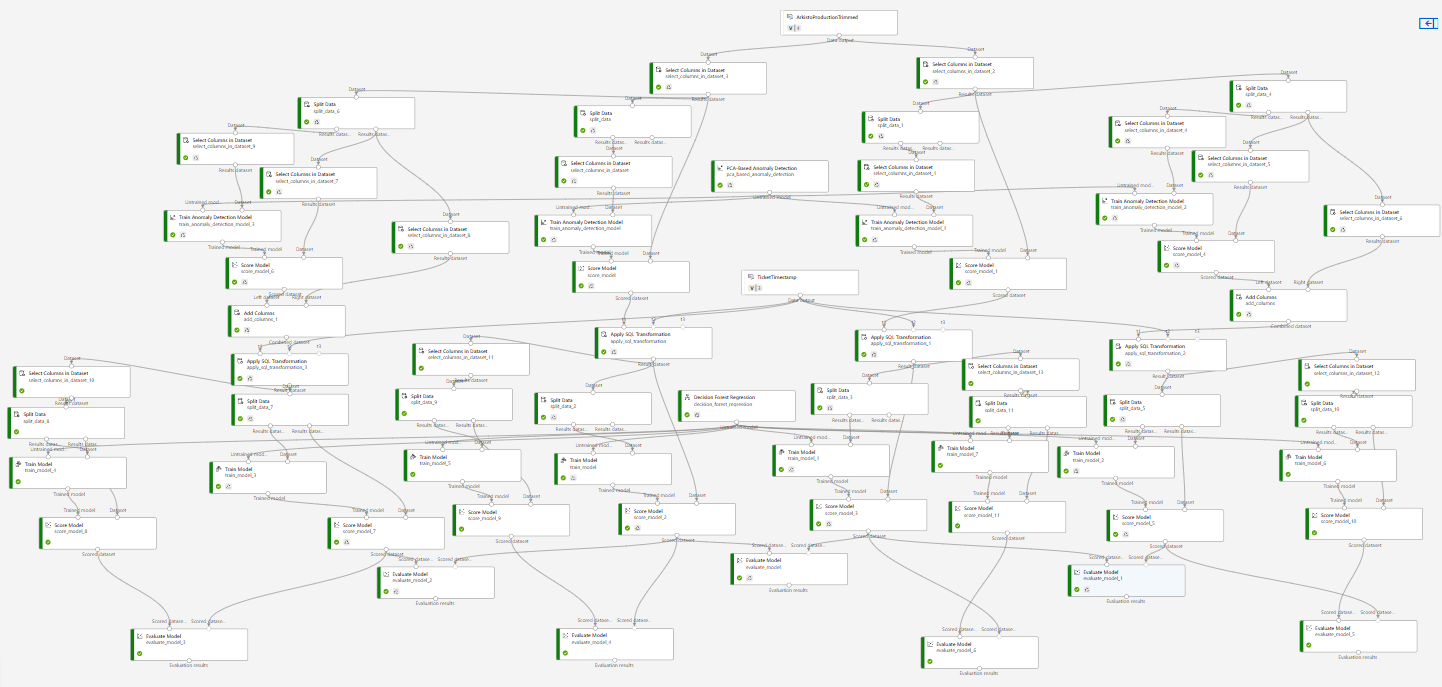
\includegraphics[width=150mm]{./appendices/pipeline-draft}
    \caption{TODO: Pipeline in all its glory. Find a better place and edit caption.
    \label{fig:pipeline draft}}
\end{figure}

%% TODO:
\todo{Explain a bit the contents of these phases. Intro to next subsections.}


%% ************************************************************************************************************


\subsection{Time frame compression and statistical features}\label{subsec:pipe-timeframe-compression-and-statistics}
To avoid the problem with random delay
between log rows and technical ticket timestamps,
as stated in the section~\ref{subsec:bg-random-delay},
log rows were grouped by time stamp
into certain time frame groups %% TODO: explain in more detail than in background
with a method we call \enquote{time frame compression},

%% TODO: Is there anything to refer to??? If exists, move to background.
This means that
in order to eliminate the effects of random delay
we compress some features in certain time frame
which is at least as long as the longest estimated delay.
Simply put,
if we count possible anomalies during one hour of log,
we cannot compare this number to actual tickets received
at the same hour or the next.
What we can do,
with time frame compression,
is that we count some statistical values of anomaly estimates,
for example, the mean and median values of a week,
and then compare these numbers with the tickets received
during the same week.



%% TODO: combination with ticket data. SQL queries
\begin{itcomment}
    This part explains some statistical features used when starting regression training
    in hybrid ML phase 2.
    These features consist of both log row amounts
    and PCA-component output values.
    All these values are grouped together in timescales.
\end{itcomment}

%% ************************************************************************************************************


\subsection{Unconventional training approach}\label{subsec:pipe-unconventional-training}

As stated in section~\ref{subsec:bg-machine-learning},
the approach used in this study is,
if expression is allowed, unorthodox. %% TODO! Check!
Typically,
data points used in ML algorithm training and validating
should always be different.
Acting otherwise
leads to algorithm processing with
same data it was trained with
thus creating a situation
where algorithm already knows what to do with the current data point.
If the results were validated after this
the algorithm would get unreliable score
as it had the validation data already in the training phase.
This could be compared to
giving some right answers to students
during test and scoring test results as if
no help was given.
However,
due to the nature of the study problem and contents of the data,
it was decided to test whether bending this rule
would provide better results in algorithm training.

Even though the amount of data was large enough
to cause issues with memory,
the hybrid approach and the time frame compression discussed <later in this section> %% TODO: check!
lead to significant reduction of data in phase 2.
As a general rule of thumb in ML training,
only 20--30\% of the data is used to validate the algorithm.
With the hybrid ML approach,
the validation results in phase 1
are what actually form the data used in the phase 2.
This data is further compressed to time frame groups
leading to only a few dozen data points in phase 2 ML training %% TODO: more accurate numbers?
compared to millions of rows in phase 1.

Because of the way the anomaly detection algorithms work
the over-lapping data points is not as big of an issue
as it would be with other types of algorithms
like regression algorithms. %% TODO: do they though?
This is why we could use part of the data
for training the anomaly detection algorithm as usual
and then use all of the available data for validation
without overfitting the algorithm. %% TODO: check and refer to something?
Also, because the main forecasting functionality comes in the phase 2,
overtraining %% TODO: check wording
in phase 1 may not cause issues. %% TODO: phrasing?

To verify if this unconventional training method gives good results without issues,
the trained algorithms were tested with new production data
that had zero overlapping data points with training and validation data.
This way we were able to compare different training approaches
to determine the best overall pipeline.



%% ************************************************************************************************************



%% TODO: Mention that data splits in phase 1 have to be un-random
%% Otherwise, possible anomaly values used in phase 2 would be randomly included
%% Data in phase 1 need to be chronological!


%% TODO: Results: Feature Hashing runs out of memory in Model Training with full data (unconventional training)
%% Trying with smaller splits, which, once again, reduces data amount.


%% ************************************************************************************************************


\subsection{Memory issues and limitations}\label{subsec:pipe-memory-issues}
Memory is crucial resource in ML training.
Algorithms take multiple steps while iterating the data
and intermediate results are stored in the RAM rather than on the disk.
%% TODO: something more to say or back that up?
While building ML pipeline in Azure ML studio,
a memory issue emerged
that affected several components
and caused serious limitations
in terms of usable components and data size.
Due to the time limits of this study
this issue was not resolved
and the problem behind it was not found.
As several conditions
considering the environment costs
were already issued by the company,
the issue was supposed to be linked with
compute instance property limitations
and thus could not be resolved without cost overruns.
However, this was not certain.

\todo{Limitations to components. List effects of this problem.}
%% TODO: limitations to components
%% limitations to data size
%% effects on choises in components?

%% ************************************************************************************************************


\subsection{Feature format for PCA-ADA}\label{subsec:pipe-pca-ada-feature-format}
%% TODO: n-gram vs pure data input
In Azure ML Studio
there is only one module selectable
for anomaly detecting,
the PCA-based anomaly detection module,
which is explained in section~\ref{subsec:bg-pca-ada}.
However,
with textual input like logs
it can be used at least in two ways.
First,
input data can be fed to
the algorithm trainer as is,
letting the PCA-based ADA component %% TODO: Explain ADA
do the work without further modifying the log rows.
This way,
the component tries to recognize the anomalies
based on all the information included in the row.
Practically this means
that the component processes data in textual format
making each row in the input
a feature as a whole
to consider.
\todo{PCA-ADA should be explained in background-section}

Second option is to
convert the textual features
into numerical n-gram features.
Each word or n-gram
is now a number of said instances found on
the row being processed,
and each row can be presented
as a sequence of numbers
indicating the number of those features.

%% TODO: N-gram theory should be explained and referred properly. Here or in background!
N-grams can in addition have a weight
based on the frequency they appear
in the entire data.
Different weights usable in Azure ML component
are listed below.

\begin{enumerate}
    \item Binary Weight
    \item TF Weight
    \item IDF Weight
    \item TF-IDF Weight
\end{enumerate}

\todo{Explain different weights and open up more Azure ML Studio PCA-component}

%% TODO: RESULTS:
%   Pure n-gram feature component using skipped
%   Only 2% of the data could be used. Not enough.
%

%% ************************************************************************************************************


\subsection{Anomaly probability}\label{subsec:pipe-anomaly-probability}
%% TODO: PCA output
\begin{itcomment}
    Here we explain what PCA-component outputs and how the result is used in the pipeline.
\end{itcomment}

The output values of the PCA-ADA component are,
as explained in the section~\ref{subsec:bg-pca-ada},
normalized so the values range between 0 and 1.
This anomaly probability value
is the main output of hybrid ML phase 1.
Based on our initial hypothesis
that each anomalous event in the log
is linked to a real life support ticket received,
the bigger a single anomaly probability value is for a log row
the more likely that row is related to a ticket inducing event.


%% ************************************************************************************************************


\subsection{Regression based estimating}\label{subsec:pipe-regression-estimating}
%% TODO: parameters?
%% Ticket amount forecasting
\begin{itcomment}
    Here is more information about different regression algorithms
    used in ML pipeline.
    Some basic information about all of them is given so the results are understandable
    by reader in the Result section.
\end{itcomment}

\begin{enumerate}
    \item Linear regression
    \item Decision forest regression
    \item \etc
    \item \etc
\end{enumerate}



\subsection{Pipeline branching}\label{subsec:pipe-branching}

%In the methods section
%we discussed of different approaches that could be used
%to get the best results from the ML training.
In order to compare different results,
some comparable metrics are needed.
%% TODO: declare comparable metrics etc.

Several diverging points caused the pipeline to branch.
First,
the error message used to calculate the anomaly probability of a log row
had two options.
We could either use simple \textit{message},
or more verbose \textit{rawmessage}.
This textual data could be fed to the ADA-component in several forms.
Most straightforward way was using textual data without any preformatting.
Text could also be run through \enquote{Preprocess text} -component. %% TODO: Explain somewhere!
N-gram features could have been extracted from the text
and these features could have been used instead.
Instead of n-gram features,
textual data could be converted to numeric
with \enquote{Feature Hashing} -component.
After getting the ADA-component results,
the anomaly probabilities were compressed with R-code or SQL. %% TODO: ?
<This concludes the phase 1.> %% TODO: ??

In phase two,
branching of the pipeline was due to either different regression algorithms used
or comparing results without the anomaly probability values calculated in phase 1.
In practice this means
that in order to validate the results against our initial hypothesis,
we used pure statistical log data such as row count and unique job ID count
without anomaly probabilities
to determine whether anomaly metrics provided any insight regarding the ticket data.

Each branching step, or layer,
multiplies the amount of results used in final comparison
that would determine the best possible pipeline combination.
These layers are simplified in the table~\ref{tab:ml-pipeline-branching}.

\begin{table}[]
    \centering
    \begin{tabularx}{\textwidth}{|L{0.3\textwidth}|L{0.45\textwidth}|X|}
        \hline
        \textbf{Branching node}           & \textbf{Options}                                                              & \textbf{Layer count} \\ \hline
        Input text column                  & \begin{tabular}[c]{@{}l@{}}message \\ rawmessage\end{tabular}                 & 2                        \\ \hline
        Text preprocess                    & \begin{tabular}[c]{@{}l@{}}Yes\\ No\end{tabular}                              & 2                        \\ \hline
        Numeric conversion                 & \begin{tabular}[c]{@{}l@{}}No\\ N-gram Feature\\ Feature Hashing\end{tabular} & 3                        \\ \hline
        ADA training                       & \begin{tabular}[c]{@{}l@{}}Unconventional \\ Proper\end{tabular}              & 2                        \\ \hline
        Validation without anomaly metrics & \begin{tabular}[c]{@{}l@{}}Yes\\ No\end{tabular}                           & 2                        \\ \hline
        Regression algorithms &
        \begin{tabular}[c]{@{}l@{}}Decision forest regression \\ Boosted decision tree regression \\ Neural Network Regression \\ Linear regression\end{tabular} &
        4 \\ \hline
    \end{tabularx}
    \caption{Pipeline divergent layers}
    \label{tab:ml-pipeline-branching}
\end{table}

The divergent count implies the number of branches
diverging from the previous component.
The total count of branch ends, or leaves,
would then be the multiplication of all divergent counts,
totaling to 192 comparable pipeline combinations.
Moreover,
n-gram feature extraction and feature hashing
have several tunable parameters
that strongly influence the end results of the algorithm training.
To reduce this amount when considering the best possible pipeline,
we simplified this by narrowing down the options
based on initial test run results of some of the divergent options.

For example,
n-gram feature component suffered greatly from the memory problem %% TODO: refer to it?
and the data amount that the \textit{Extract N-Gram Features from Text} -component
was able to handle only 2\% of the original data amount.
This was deemed as too small amount for training
as it would be extremely likely with 98\% of the data skipped
that also possible rows relevant to the ticket anomalies
would get trimmed out.



%% TODO: unorganized text below!

%% TODO: Next up is outdated
%
%Usually <with usual ml methods> the estimates
%created using ML algorithms
%are formed based on the certain features
%presented on a one element of the data,
%or on one row.
%This means that in typical case,
%there is one column in the data
%given to the ML algorithm
%that is removed from the training data
%and this column value is what algorithm
%aims to predict.
%
%In this study case, however,
%data does not contain clear values
%that are being estimated
%and that can be used as comparison.
%
%\begin{tabular}{cccc}
%    LOG\_DATA \\
%    a=date & b=msg & c=\etc & \\
%    a & b & c & n1 \\
%    a & b & c & n2 \\
%    a & b & c & n3 \\
%    a & b & c & n4
%\end{tabular}
%
%\begin{tabular}{c}
%    EFECTE\_DATA \\
%    A YYYY.MM.DD hh:mm:ss \\
%    B YYYY.MM.DD hh:mm:ss \\
%    C YYYY.MM.DD hh:mm:ss \\
%    D YYYY.MM.DD hh:mm:ss \\
%    E YYYY.MM.DD hh:mm:ss
%\end{tabular}
%\\
%n1 = SUM(AB) \\
%n2 = SUM(C) \\
%n3 = SUM(DE) \\
%=> \\
%We could try to predict nx
%but usually this is done
%by making estimate based on
%a, b and c.
%Instead,
%we aim to estimate the sum of events
%in timeframe.
%We should also skip event instances
%that are close to each other
%to avoid counting multiple values
%linked to same error
%as different possible ticket creators.




\clearpage